\documentclass[11pt]{article}
\usepackage{amsmath,amssymb, amsthm, marvosym, permute, extsizes}
\usepackage{siunitx, graphicx, float, enumitem, adjustbox, hyperref, bm}
\usepackage{microtype, dsfont}
\usepackage[normalem]{ulem}
\usepackage{braket}
\usepackage[T1]{fontenc}
\usepackage[utf8]{inputenc}
\usepackage[justification=centering]{caption}
\usepackage{lmodern}
\usepackage{mhchem}
\usepackage{gensymb}
\usepackage[T1]{fontenc}
\usepackage[a4paper,margin=2.5cm]{geometry}
\usepackage[icelandic]{babel}
\usepackage{tikz}
\newcommand{\explain}[2]{\underbrace{#1}_\textrm{$#2$}}
\usepackage{minted}
\usemintedstyle{perldoc}
\parindent = 0pt
\usepackage{fancyhdr}
    \pagestyle{fancy}
    \headheight=32pt
    \lhead{Háskóli Íslands\\Raunvísindadeild}
    \rhead{Verkleg Eðlisfræði}
\title{{\Huge Atómkraftasjá}}
\author{Emil Gauti Friðriksson \& Garðar Árni Skarphéðinsson}
\date{Apríl 2019 \\
\vspace{5cm}

\includegraphics[width = .6\textwidth]{HIlogo1.png}}

\begin{document}

\maketitle
\thispagestyle{empty}

\newpage

\section{Inngangur}
Atómkraftasjá (e. Atomic Force Microscope), eða AFM, er tæki sem er notað til þess að taka myndir af yfirborðum á nanóskala með mikilli nákvæmni. Örsmár oddur er færður eftir yfirborði efnisins, annað hvort í beinni snertingu við efnið eða rétt fyrir ofan það. Lögun yfirborðsins er greind út frá kröftunum sem verka á oddinn og sveigja brettið sem hann er festur undir. Í þessari tilraun var atómkraftasjá notuð til þess að mæla van der Waals krafta og teikna upp mynd af bæði paladín ($Pd$) og safír ($Al\ce{_{2}}O\ce{_3}$) húðum. Forrit var síðan notað til þess að skoða hrjúfleika húðarinnar. \\

\section{Pd/MgO greining}
Atómkraftasjáin er notuð í þeim tilgangi að skoða hið góðkunna sýni {\tt KEN001} sem er þunn palladín húð ræktuð á magnesíum-oxíð við \ang{100}C. Mynd~\ref{fig:Pd/MgO fjarmynd} sýnir grófa mynd af yfirborðinu.

\begin{figure}[H]
  \centering
    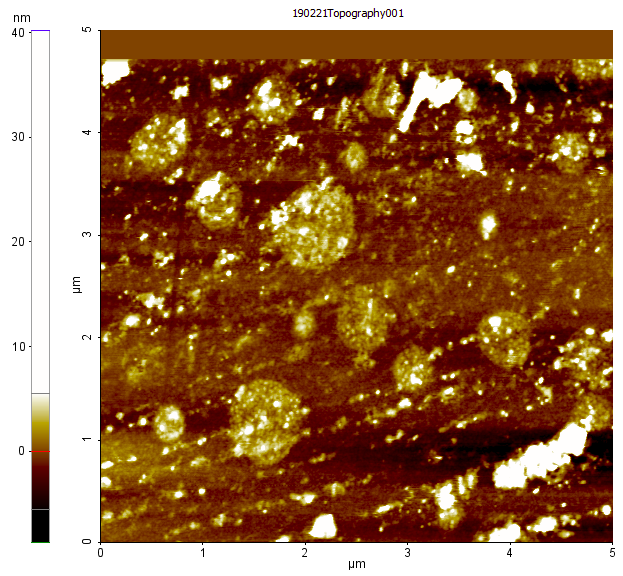
\includegraphics[width=100mm]{Ken01/Screenshot1.png}
    \caption{$5$x$5$ $\mu m$ hæðarmynd af Pd/MgO húð sem ræktuð var við \ang{100}C. Ljósir litir eru notaðir til að tákna hóla og dökkir litir tákna dali.}
    \label{fig:Pd/MgO fjarmynd}
\end{figure}

Við sjáum tvo einkennandi hluti við mynd~\ref{fig:Pd/MgO fjarmynd}

\begin{itemize}
    \item Hvítar skrámur - Þetta er líklegast skrámur eftir lélega meðhöndlun á sýninu.
    \item Skífulaga hólar - Afbrigðileg uppröðun palladíns við ræktun.
\end{itemize}
Við getum metið kornastærð húðarinnar gróflega út frá mynd~\ref{fig:Pd/MgO fjarmynd} en hún virðist vera af stærðargráðunni \sim\SI{100}{nm}.\\


Við skoðum einnig {\tt KEN004} sýnið sem er palladín húð ræktuð á magnesíum-oxíð við \ang{400}C en þar væntum við þess að skífulaga hólarnir séu smærri sökum þess að palladín atómin hafa meiri hreyfiorku þegar þau lenda á undirlaginu og mynda þar af leiðandi jafndreifðara/flatara yfirborð.


\begin{figure}[H]
  \centering
  \begin{minipage}[b]{0.48\textwidth}
    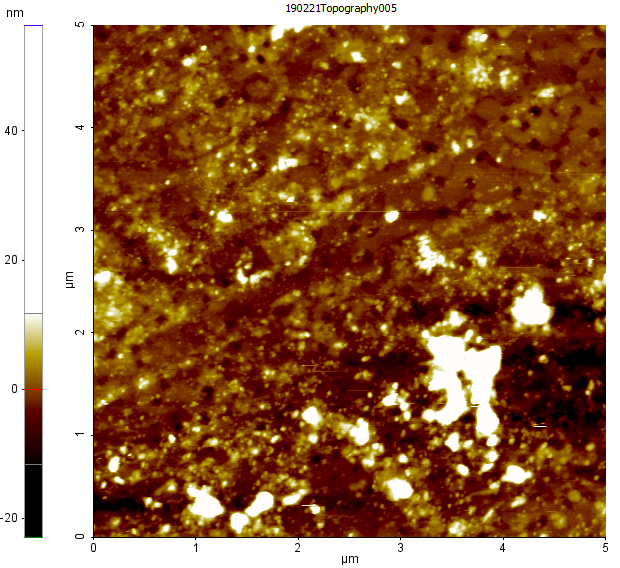
\includegraphics[width=\textwidth]{KEN002/Screenshot3.png}
    \caption{$5$x$5$ $\mu m$ mynd af Pd/MgO húð sem ræktuð var við \ang{400}C.}
    \label{fig:fjar400}
  \end{minipage}
  \hfill
  \begin{minipage}[b]{0.48\textwidth}
    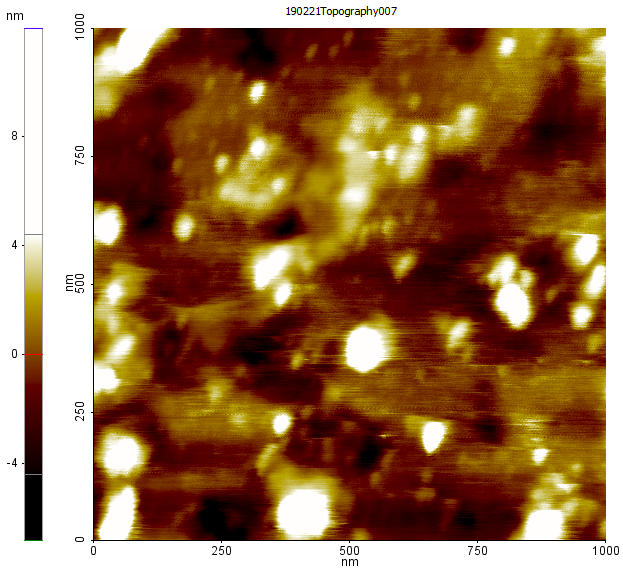
\includegraphics[width=\textwidth]{KEN002/Screenshot4.png}
    \caption{$1$x$1$ $\mu m$ mynd af Pd/MgO húð sem ræktuð var við \ang{400}C.}
    \label{fig:naer400}
  \end{minipage}
\end{figure}

Eins og sést á myndum  \ref{fig:fjar400} og \ref{fig:naer400} þá virðist kornastærð {\tt KEN004} sýnisins vera mjög sambærileg við stærðina í {\tt KEN001} eða um það bil \SI{100}{nm}. Við sjáum einnig að sú ályktun að hólarnir yrðu minni á {\tt KEN004} reyndist rétt, og er yfirborðið talsvert flatara.

%Miiiiklu minni hólar. Svipuð kornastærð. Ræktun við hærra hitastig gefur meira smooth yfirborð. Held hvíta dótið þarna sé bara eh óhreinindi/klessa.

\section{Greining á Safírhúð ($Al\ce{_{2}}O\ce{_3}$)}

Við skoðum nú þrjár mismunandi safírhúðir, og er eini munurinn á þeim er hvaða plan kristalsins er samsíða yfirborði húðarinnar. Við skoðum a-, c- og m-plön, en legu þeirra miðað við einingargrind safírs sést hér á mynd~\ref{fig:Safir plon}.

\begin{figure}[H]
  \centering
    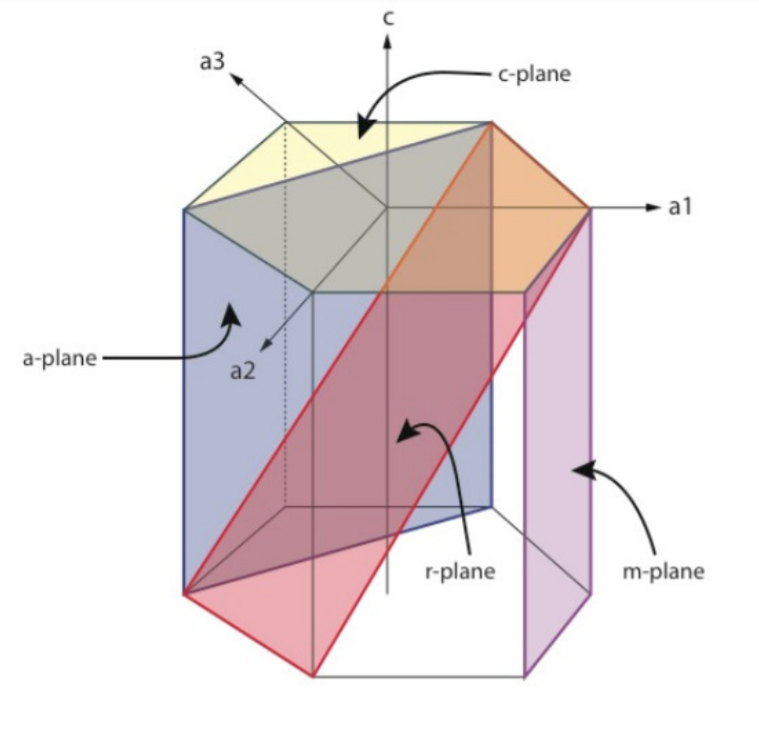
\includegraphics[width=80mm]{Safir_planes.PNG}
    \caption{Kristalsplön safírs.}
    \label{fig:Safir plon}
\end{figure}

\subsection*{Safír a-plan}

\begin{figure}[H]
  \centering
    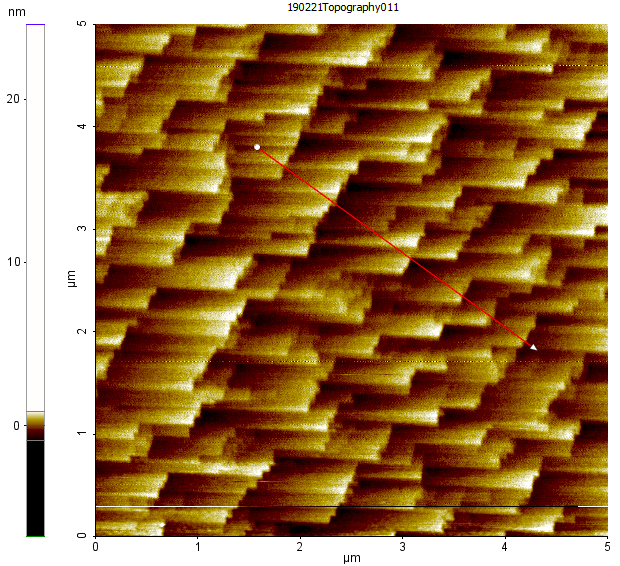
\includegraphics[width=145mm]{Safir-A/Screenshot6.png}
    \caption{$5$x$5$ $\mu m$ hæðarmynd af safír húð sem með a-plan samsíða yfirborði.}
    \label{fig:A-plan fjarmynd}
\end{figure}

\begin{figure}[H]
  \centering
    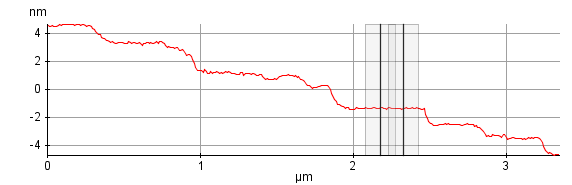
\includegraphics[width=145mm]{Safir-A/190221Topography011_Line_slanted}
    \caption{Hæð yfirborðsins eftir rauðu línunni á mynd~\ref{fig:A-plan fjarmynd}}
    \label{fig:A-plan línurit fjarmynd}
\end{figure}

Af myndum~\ref{fig:A-plan fjarmynd} og~\ref{fig:A-plan línurit fjarmynd} sést hvar plön kristalsins liggja ofan á hverju öðru. Á yfirborðinu myndast því þessi u.þ.b. $\SI{2}{nm}$ þrep þar sem plönin enda. Hvert þrep virðist vera um $\SI{0.5}{\mu m}$ á lengd þannig að hornið sem þrepin mynda eru um það bil $\arctan(\SI{2}{nm}/\SI{0.5}{\mu m}) = 0.23\degree$.


\subsection*{Safír c-plan}

\begin{figure}[H]
  \centering
    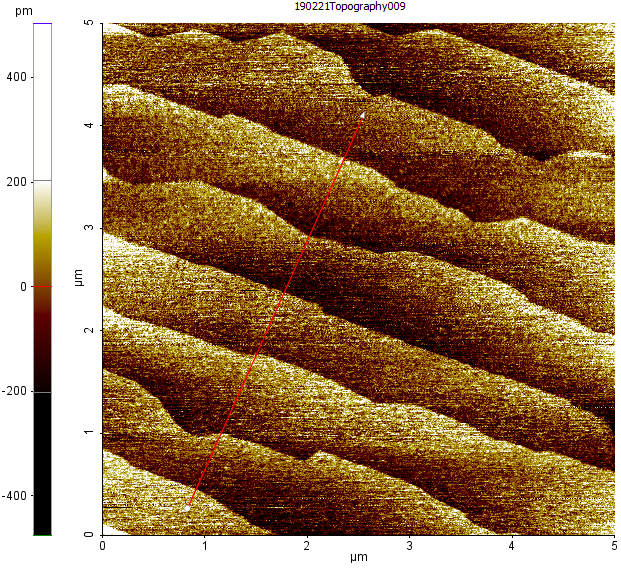
\includegraphics[width=145mm]{SAFIR-C/Screenshot_C.png}
    \caption{$5$x$5$ $\mu m$ hæðarmynd af safír húð sem með c-plan samsíða yfirborði.}
    \label{fig:C-plan fjarmynd} 
\end{figure}

\begin{figure}[H]
  \centering
    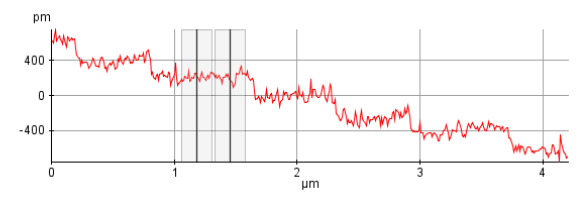
\includegraphics[width=145mm]{SAFIR-C/C_plan-linurit.PNG}
    \caption{Hæð yfirborðsins eftir rauðu línunni á mynd~\ref{fig:C-plan fjarmynd}}
    \label{fig:C-plan línurit fjarmynd}
\end{figure}

Af myndum~\ref{fig:C-plan fjarmynd} og~\ref{fig:C-plan línurit fjarmynd} sést svipaður þrepastrúktúr og á myndum~\ref{fig:A-plan fjarmynd} og~\ref{fig:A-plan línurit fjarmynd}. Hér virðist þrepin einnig vera um $\SI{0.5}{\mu m}$ á lengd en hæð þeirra er nú um það bil $\SI{200}{pm}$. Hornið sem þrep plananna mynda er því ca. $\arctan(\SI{200}{pm}/\SI{0.5}{\mu m}) = 0.023\degree$.

\subsection*{Safír m-plan}

\begin{figure}[H]
  \centering
    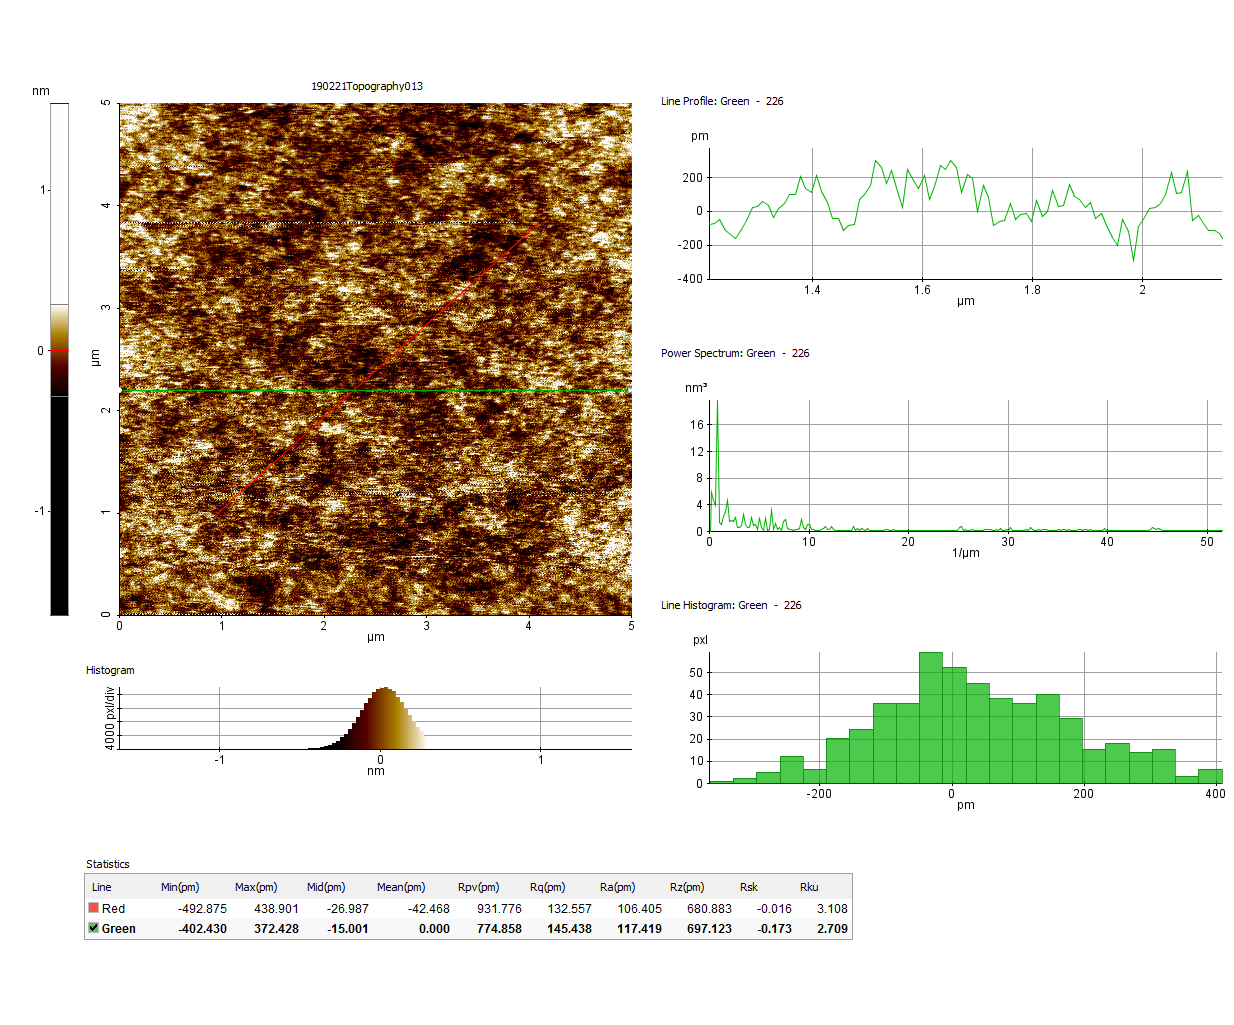
\includegraphics[width=130mm]{Safir-M/190221Topography013.png}
    \caption{$5$x$5$ $\mu m$ hæðarmynd af safír húð sem með m-plan samsíða yfirborði. Efsta grafið sýnir hæð yfirborðsins eftir grænu línunni á myndinni.}
    \label{fig:m-plan fjarmynd}
\end{figure}

Á mynd~\ref{fig:m-plan fjarmynd} sést mjög gróft yfirborð og ekki má greina nein augljós þrep eins og fyrir hinar tvær safír húðirnar. 


\section{Kvörðun}

\begin{figure}[H]
    \centering
    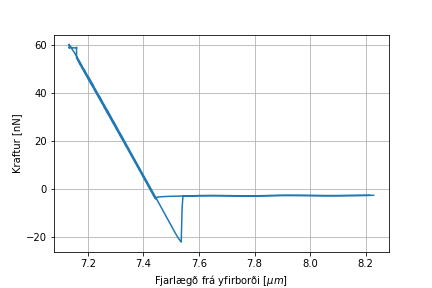
\includegraphics{forceDist.png}
    \caption{Kraftur sem fall af fjarlægð frá yfirborði}
    \label{fig:forceDist}
\end{figure}
Athugum að við fáum öðruvísi kúrfu þegar nálin er að nálgast yfirborðið og þegar hún fjarlægist það, það kemur til vegna van der Waals krafta sem gerir það að verkum að við mælum neikvæðan kraft. Þetta er í samræmi við fræði úr fyrirlestri.
\end{document}
